\subsection{Mechanics}

The final mechanical structure of the robot is composed of \textbf{two dodecagonal wooden platforms}: a \textbf{base platform} and an \textbf{upper platform}, connected by four vertical wooden columns. This simplified configuration was adopted after removing the initially planned intermediate layer, which had interfered with wheel clearance.

The \textbf{base platform} is the core of the system and holds \textbf{all the critical mechanical and electronic components}:

\begin{itemize}
    \item On the \textbf{underside}, we mounted the \textbf{three DC motors}, each connected to a \textbf{58 mm omnidirectional wheel} in a triangular layout to enable holonomic movement. The \textbf{motor drivers} are also fixed on this side, close to the motors, to reduce wiring length and improve accessibility.
    \item On the \textbf{upper side} of the same platform, we installed the \textbf{microcontroller}, \textbf{sensor wiring}, \textbf{power distribution boards}, and the \textbf{battery}. A vertical plastic panel helps organize the electronics, and the ultrasonic sensors are positioned around the base perimeter on alternating sides.
\end{itemize}

The \textbf{upper platform} is structurally intended to support \textbf{other modules}, such as the ticket dispenser or user interface components. It is fixed to the columns and aligned with the base to maintain symmetry and provide vertical expansion space.

\begin{figure}[H]
    \centering
    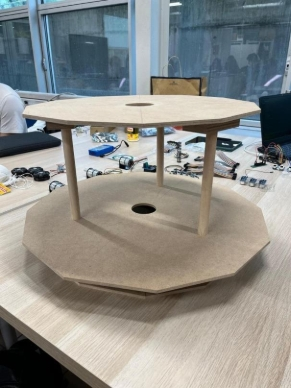
\includegraphics[width=0.7\linewidth]{../ReportMovementModule/images/Aspose.Words.728084da-df58-4b9d-a372-f65cffbdb23d.023.jpeg}
    \caption{Final Mechanical Structure}
\end{figure}

All mechanical parts were fabricated using MDF panels and wooden supports, based on our technical drawings and 3D model. The final structure provides a \textbf{stable, modular, and compact skeleton} for the movement module, optimized for both functionality and future adaptability.

\subsubsection{Movement System}

The triangular configuration of the three omnidirectional wheels provides several key advantages:

\begin{itemize}
    \item \textbf{Holonomic movement}: The robot can move in any direction and rotate in place without needing to change orientation first
    
    \item \textbf{Simplified control}: With three wheels at 120° intervals, the inverse kinematics calculations become more straightforward
    
    \item \textbf{Mechanical stability}: The weight distribution across three points provides good balance while minimizing the number of components
    
    \item \textbf{Improved maneuverability}: The design allows for efficient navigation in tight spaces, crucial for the robot's intended environment
\end{itemize}

\subsubsection{Structural Adaptations}

During assembly and testing, we made several mechanical adaptations to optimize performance:

\begin{itemize}
    \item \textbf{Removal of lower platform}: To increase wheel clearance and improve movement reliability
    
    \item \textbf{Addition of cotton padding}: For both aesthetic effect and to protect internal components
    
    \item \textbf{Reinforcement of column connections}: To ensure rigidity during rapid movements and direction changes
    
    \item \textbf{Redistribution of component weights}: For better balance and stability during rotation
\end{itemize}

\begin{figure}[H]
    \centering
    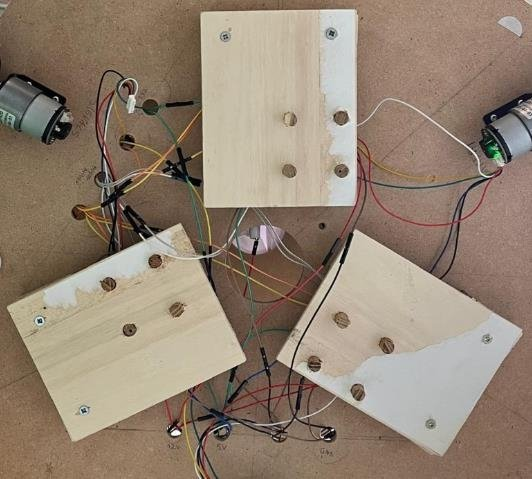
\includegraphics[width=0.7\linewidth]{../ReportMovementModule/images/Aspose.Words.728084da-df58-4b9d-a372-f65cffbdb23d.025.jpeg}
    \caption{Final Structural Configuration}
\end{figure}

These mechanical features come together to create a reliable platform that successfully fulfills the movement requirements of our social robot design.
